\documentclass{article}
  %----------------------------------------------------------------------------------------
%	Author:	WangYifu
%	Create Date:	2017-02-14
%	Last Modify:	2018-09-01
%----------------------------------------------------------------------------------------
\usepackage[T1]{fontenc}
\usepackage{fourier}
\usepackage[english]{babel}
\usepackage{amsmath,amsfonts,amsthm}
\usepackage{geometry}
\usepackage{fancyhdr}
\usepackage{listings}
\usepackage{color}
\usepackage[yyyymmdd]{datetime}
\usepackage{graphicx}
\usepackage{float}
\usepackage{titling}
\usepackage{titlesec}
%-------------------------------%
%          Page Style           %
%-------------------------------%
\pagestyle{fancyplain}
\fancyhead{}
\fancyfoot[L]{}
\fancyfoot[C]{}
\fancyfoot[R]{\thepage}
\renewcommand{\headrulewidth}{0pt}
\renewcommand{\footrulewidth}{0pt}
\setlength{\headheight}{13.6pt}
\textwidth=6.5in
\textheight=9.0in
\headsep = 0.1in
\renewcommand{\baselinestretch}{1.2}
\geometry{a4paper,left=2cm,right=2cm,top=2cm,bottom=2cm}

%-------------------------------%
%           Font Size           %
%-------------------------------%
\newcommand{\erhao}{\fontsize{22.1pt}{\baselineskip}\selectfont}
\newcommand{\sanhao}{\fontsize{16.1pt}{\baselineskip}\selectfont}
\newcommand{\sihao}{\fontsize{14.1pt}{\baselineskip}\selectfont}
\newcommand{\xiaosi}{\fontsize{12.1pt}{\baselineskip}\selectfont}
\newcommand{\wuhao}{\fontsize{10.5pt}{\baselineskip}\selectfont}
\newcommand{\setFontSize}[1]{\fontsize{#1}{\baselineskip}\selectfont}
\titleformat{\section}{\sanhao\bfseries}{$\bullet$}{5pt}{}

%-------------------------------%
%             Title             %
%-------------------------------%
\newcommand{\horrule}[1]{\rule{\linewidth}{#1}}
\renewcommand{\dateseparator}{ - }
\def\Assignment{Assignment Title}
\title{
\vspace{-2cm}
\normalfont \normalsize
\textsc{Washington University in St. Louis} \\ [0pt]
\horrule{1pt} \\[0.4cm]
\huge {\bf\Assignment}
}
\author{467261 - Yifu Wang}
\date{\normalsize\today\\\horrule{1pt} \\[0.5cm]}

%-------------------------------%
%           TableList           %
%-------------------------------%
\newcommand{\deflabel}[1]{#1\hfill}
\newenvironment{tlist}[1]{
	\begin{list}{}{
			\settowidth{\labelwidth}{\bf#1}
			\setlength{\leftmargin}{\labelwidth}
			\addtolength{\leftmargin}{\labelsep}
			\renewcommand{\makelabel}{\bf\deflabel}}}{
	\end{list}
}

%-------------------------------%
%             Code              %
%-------------------------------%
\definecolor{gray}{RGB}{191,191,191}
\definecolor{dkgreen}{RGB}{96,139,78}
\definecolor{mauve}{RGB}{206,145,120}

\lstset{ %
	language=C++,                % the language of the code
	% basicstyle=\textheight,           % the size of the fonts that are used for the code
	numbers=left,                   % where to put the line-numbers
	numberstyle=\color{black},  % the style that is used for the line-numbers
	stepnumber=0,                   % the step between two line-numbers. If it's 1, each line 
	% will be numbered
	numbersep=5pt,                  % how far the line-numbers are from the code
	backgroundcolor=\color{gray},      % choose the background color. You must add \usepackage{color}
	showspaces=false,               % show spaces adding particular underscores
	showstringspaces=false,         % underline spaces within strings
	showtabs=false,                 % show tabs within strings adding particular underscores
	frame=false,                   % adds a frame around the code
	rulecolor=\color{gray},        % if not set, the frame-color may be changed on line-breaks within not-black text (e.g. commens (green here))
	tabsize=2,                      % sets default tabsize to 2 spaces
	captionpos=b,                   % sets the caption-position to bottom
	breaklines=true,                % sets automatic line breaking
	breakatwhitespace=false,        % sets if automatic breaks should only happen at whitespace
	keywordstyle=\color{blue},          % keyword style
	commentstyle=\color{dkgreen},       % comment style
	stringstyle=\color{mauve},         % string literal style
}

  \def\Assignment{CSE 547T - HW3}
  \usepackage[pdf]{graphviz}
\begin{document}
\maketitle
\begin{tlist}{10}
	\item[3.38 (c)]\
	\begin{center}
		\begin{tabular}{c|c|c}
			  & $\sigma(q,a)$ & $\sigma(q,b)$ \\\hline
			1 & \{1,2\}       & \{2\}         \\
			2 & \{3\}         & \{2\}         \\
			3 & \{3\}         & \{3,4\}       \\
			4 & $\emptyset$   & $\emptyset$   \\
		\end{tabular}
	\end{center}
	\begin{figure}[H]\centering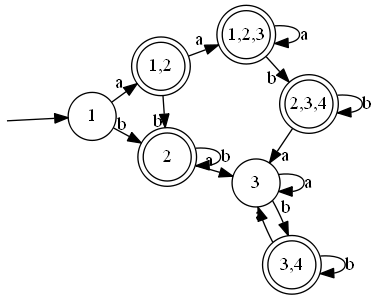
\includegraphics[scale=.6]{g1.png}\end{figure}
	\item[3.38 (d)]\
	\begin{center}
		\begin{tabular}{c|c|c}
			  & $\sigma(q,a)$ & $\sigma(q,b)$ \\\hline
			1 & \{2\}         & $\emptyset$   \\
			2 & $\emptyset$   & \{3\}         \\
			3 & \{1,4,5\}     & $\emptyset$   \\
			4 & \{5\}         & $\emptyset$   \\
			5 & \{1\}         & $\emptyset$   \\
		\end{tabular}
	\end{center}
	\begin{figure}[H]\centering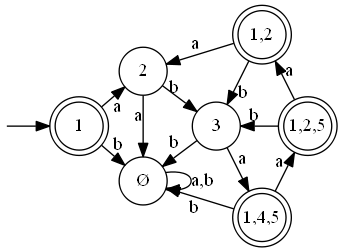
\includegraphics[scale=.6]{g2.png}\end{figure}
	\item[2.22 (a)]
	\begin{tlist}{2}
		\item[$\bullet$]
		Assume $L$ is accepted by an FA with $m$ states, where $m\in\mathbb{N}^+$.
		\item[$\bullet$]
		Consider string $s=a^mba^{2m}$, since $|s|>m$, by pumping lemma we should be able to find such a 3-tuple $(u,v,w)$ where $s=uvw$ and $v\neq\Lambda$ that $uv^iw\in L\ \forall\ i\in\mathbb{N}$.
		\item[$\bullet$]
		Firstly, $v$ couldn't contains $b$, since all string in $L$ contains only one $b$. So $v$ should be contained either in $a^m$ part or $a^{2m}$ part. But then the variation of $i$ will break the proportion between this two parts.
		\item[$\bullet$]
		Thus $L$ can't be accepted by an FA.
	\end{tlist}
	\item[2.22 (b)]
	\begin{tlist}{2}
		\item[$\bullet$]
		Assume $L$ is accepted by an FA with $m$ states, where $m\in\mathbb{N}^+$.
		\item[$\bullet$]
		Consider string $s=a^mb^ma^{2m+1}$, since $|s|>m$, by pumping lemma we should be able to find such a 3-tuple $(u,v,w)$ where $s=uvw$ and $v\neq\Lambda$ that $uv^tw\in L\ \forall\ t\in\mathbb{N}$.
		\item[$\bullet$]
		Firstly, let's divide $s$ into 3 parts, which are $a^m$, $b^m$ and $a^{2m+1}$. Obviously $v$ can only be contained in one part, otherwise the variation of $i$ will destroy this 3-parts pattern. Secondly, $v$ can't be contained in the first two parts, since when $t$ goes up, $i+j$ will exceed $k$ eventually. But again, $v$ can't be contained in part 3 either. Since $|v|\neq 0$, thus when we take $t=0$, we will get $i+j=k$ which is not acceptable.
		\item[$\bullet$]
		Thus $L$ can't be accepted by an FA.
	\end{tlist}
\end{tlist}
\end{document}